\documentclass[twoside,twocolumn]{article}

\usepackage{blindtext} % Package to generate dummy text throughout this template 
\usepackage{graphicx}
\usepackage[sc]{mathpazo} % Use the Palatino font
\usepackage[T1]{fontenc} % Use 8-bit encoding that has 256 glyphs
\linespread{1.05} % Line spacing - Palatino needs more space between lines
\usepackage{microtype} % Slightly tweak font spacing for aesthetics

\usepackage[english]{babel} % Language hyphenation and typographical rules

\usepackage[hmarginratio=1:1,top=32mm,columnsep=20pt]{geometry} % Document margins
\usepackage[hang, small,labelfont=bf,up,textfont=it,up]{caption} % Custom captions under/above floats in tables or figures
\usepackage{booktabs} % Horizontal rules in tables
\usepackage{graphicx}
\usepackage{lettrine} % The lettrine is the first enlarged letter at the beginning of the text

\usepackage{enumitem} % Customized lists
\setlist[itemize]{noitemsep} % Make itemize lists more compact

\usepackage{abstract} % Allows abstract customization
\renewcommand{\abstractnamefont}{\normalfont\bfseries} % Set the "Abstract" text to bold
\renewcommand{\abstracttextfont}{\normalfont\small\itshape} % Set the abstract itself to small italic text

\usepackage{titlesec} % Allows customization of titles

\titleformat{\section}[block]{\large\scshape\centering}{\thesection.}{1em}{} % Change the look of the section titles
\titleformat{\subsection}[block]{\large}{\thesubsection.}{1em}{} % Change the look of the section titles

\usepackage{fancyhdr} % Headers and footers
\pagestyle{fancy} % All pages have headers and footers
\fancyhead{} % Blank out the default header
\fancyfoot{} % Blank out the default footer
\fancyhead[C]{Comparativa Business Analytics vs Business Intelligence $\bullet$ Marzo 2022 $\bullet$ } % Custom header text
\fancyfoot[RO,LE]{\thepage} % Custom footer text

\usepackage{titling} % Customizing the title section

\usepackage{hyperref} % For hyperlinks in the PDF

%----------------------------------------------------------------------------------------
%	TITLE SECTION
%----------------------------------------------------------------------------------------
\providecommand{\keywords}[1]{
  \small	
  \textbf{\textit{\quad \quad Keywords: }} #1}

\providecommand{\pclave}[1]{
  \small	
  \textbf{\textit{\quad \quad Palabras Clave: }} #1}

%Idiomas: \selectlanguage{english} \selectlanguage{spanish}

\begin{document}

\title{Trabajo Encargado N°1: Comparativa Business Analytics vs Business Intelligence}

\begin{titlepage}
\begin{figure}[htb]
\begin{center}

\includegraphics[width=5cm]{imagenes/logo.png}
\end{center}
\end{figure}
\vspace*{-0.25in}
\begin{center}
\large{UNIVERSIDAD PRIVADA DE TACNA}\\
\vspace*{-0.025in}
INGENIERIA DE SISTEMAS  \\	

\vspace*{0.5in}
\begin{large}
TITULO:\\
\end{large}

\vspace*{0.1in}
\begin{Large}
\textbf{Comparativa Business Analytics vs Business Intelligence} \\
\end{Large}

\vspace*{0.3in}
\begin{Large}
\textbf{CURSO:} \\
\end{Large}

\vspace*{0.1in}
\begin{large}
Inteligencia de Negocios\\
\end{large}

\vspace*{0.3in}
\begin{Large}
\textbf{DOCENTE:} \\
\end{Large}

\vspace*{0.1in}
\begin{large}
 Ing. Patrick Cuadros Quiroga\\
\end{large}

\vspace*{0.2in}
\vspace*{0.1in}
\begin{large}

Integrantes: \\
\begin{flushleft}
Maldonado Cancapi, Carlos Alejandro\hfill(2018000660) \\
Huillca Aroni, Alfredo\hfill(2018060903)\\
Anahua Huayhua, Jenny Karen\hfill(2018062150)\\
Coloma Colquehuanca, Kiara\hfill(2018062218)\\

\end{flushleft}
\end{large}

\vspace*{0.1in}
\begin{large}
Tacna - Perú\\
2022
\end{large}
\end{center}
\end{titlepage}

\setlength{\droptitle}{-4\baselineskip} % Move the title up

\pretitle{\begin{center}\Huge\bfseries} % Article title formatting
\posttitle{\end{center}} % Article title closing formatting
\title{Comparativa Business Analytics vs Business Intelligence} % Article title

\date{\today} % Leave empty to omit a date                     
\renewcommand{\maketitlehookd}{%

}

%----------------------------------------------------------------------------------------



% Print the title
\maketitle

%----------------------------------------------------------------------------------------
%	ARTICLE CONTENTS
%----------------------------------------------------------------------------------------

\section{Resumen}
En los últimos años, las organizaciones han recurrido cada vez más a soluciones de 
software avanzadas para administrar las cargas de trabajo, mantener la rentabilidad y
asegurad la competitividad dentro de sus respectivas industrias. Si bien hay varias opciones de negocios
(BA) son posiblemente las soluciones de administración de datos más implementadas. Los analistas de negocios y los 
compradores de software a menudo preguntan cuáles son las diferencias clave entre las inteligencia de negocios y los
análisis de negocios.

%------------------------------------------------

\section{Abstract}
In recent years, organizations have increasingly turned to advanced software solutions to 
manage workloads, maintain profitability and ensure competitiveness within their respective
 industries. While there are several options 
 available, business intelligence tools (BI) and business analytics tools (BA) are 
 arguably the most widely implemented data management solutions. Business analysts
  and software buyers alike often ask what are the key differences between business intelligence vs business analytics.






%------------------------------------------------
\section{Introduccion}

La gestión de una organización se fundamenta en tomar decisiones adecuadas respecto a 
clientes, productos, empleados, proveedores y procesos de negocio. Por lo tanto, es necesario 
tener mecanismos que den soporte a una toma de decisiones eficiente. En los últimos años, ha 
emergido una nueva forma de competir que se fundamenta en tomar decisiones basadas en 
datos y evidencias dejando atrás la intuición. Esta forma de competir combina diferentes 
estrategias para generar valor de negocio: business intelligence (BI), business analytics y big 
data. No extraño que los CIO de las principales empresas del mundo destaquen que su principal 
prioridad tecnológica son este tipo de iniciativas. Así, la explotación de la información en el 
contexto de las organizaciones ha pasado de ser una necesidad a una prioridad de máxima 
relevancia. El objetivo es poder tomar mejores y más rápidas decisiones informadas de negocio.
\begin{center}

\end{center}

\section{Desarrollo}

\subsection{Business Intelligence}
\subsubsection{Concepto}
Business Intelligence, en español, Inteligencia Empresarial o Inteligencia de Negocios. Surge en 1996 cuando Gartner Group, en uno de sus reportes, manifestó que “Se requiere intuición para tomar decisiones correctas” y que “las herramientas de reporte, consulta y análisis de datos pueden ayudar a los usuarios de negocios a navegar a través de un mar de información para sintetizar la información valiosa que en él se encuentra”. 
El objetivo básico de la Inteligencia de Negocios es apoyar de forma sostenible y continuada a las organizaciones para mejorar su competitividad, facilitando la información necesaria para la toma de decisiones. El primero que acuñó el término fue Howard Dresner que, cuando era consultor de Gartner, popularizó Business Intelligence o BI como un término paraguas para describir un conjunto de conceptos y métodos que mejoraran la toma de decisiones, utilizando información sobre qué había sucedido (hechos). El BI examina los datos que se reportan en un formato que puede interpretarse de manera clara y rápida. Los paneles de control en tiempo real, por ejemplo, son un mecanismo de visualización muy útil, pues gracias a ellos los administradores pueden generar reportes integrales y precisos que contienen datos relevantes y procesables para tomar acción dentro de la compañía.
Algunas de las tecnologías que forman parte de la business intelligence son estas:
\begin{itemize}
    \item   Data warehouse. 
    \item   Reporting. 
    \item   Análisis OLAP (online analytical processing).
    \item   Análisis visual. 
    \item   Análisis predictivo. 
    \item   Cuadro de mando. 
    \item   Cuadro de mando integral.  
    \item   Minería de datos.  
    \item   Gestión del rendimiento. 
    \item   Previsiones.
    \item   Reglas de negocio.
    \item   Dashboards.
    \item   Integración de datos (que incluye extract, transform and load; ETL).
\end{itemize}

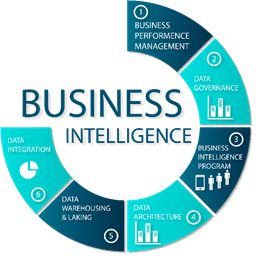
\includegraphics[width=6cm]{imagenes/img1.png}
\subsubsection{Beneficios del Business Intelligence}
\begin{itemize}
    \item   Visualizar y analizar datos con gran velocidad, eficiencia y entendimiento, todo ello con un lenguaje natural y fácil de comprender, y desde una única plataforma. 
    \item   Ofrecer información de la organización en todo momento, en cualquier lugar y desde cualquier dispositivo (PC, Móvil, Tablet). 
    \item   Crear cuadros de mando e informes específicos según las necesidades de la organización y áreas específicas, y compartir dichos informes y paneles con cualquier persona, ya sean miembros de la empresa o clientes. 
    \item   Agregar valor al negocio y a las soluciones ofrecidas a los clientes
    \item   Aprovechar los datos que generan todas las áreas para conocer tendencias, analizar distintos escenarios, obtener respuestas, etc.
    \item  Crear, manejar y mantener métricas, indicadores claves de rendimiento (key performance indicador; KPI) e indicadores claves de metas (key goal indicator; KGI) fundamentales para la empresa.
\end{itemize}

\subsubsection{Componentes de Business Intelligence}

\begin{itemize}
    \item   Fuentes de información, de las cuales partiremos para alimentar de información el datawarehouse.
    \item   Proceso ETL de extracción, transformación y carga de los datos en el datawarehouse. Antes de almacenar los datos en un datawarehouse, éstos deben ser transformados, limpiados, filtrados y redefinidos. Normalmente, la información que tenemos en los sistemas transaccionales no está preparada para la toma de decisiones. 
    \item  El propio datawarehouse o almacén de datos, con el Metadata o Diccionario de datos. Se busca almacenar los datos de una forma que maximice su flexibilidad, facilidad de acceso y administración. 
    \item   El motor OLAP, que nos debe proveer capacidad de cálculo, consultas, funciones de planeamiento, pronóstico y análisis de escenarios en grandes volúmenes de datos. En la actualidad existen otras alternativas tecnológicas al OLAP, que también desarrollaremos en el presente capítulo. 
    \item   Las herramientas de visualización, que nos permitirán el análisis y la navegación a través de los mismos. 
    
\end{itemize}
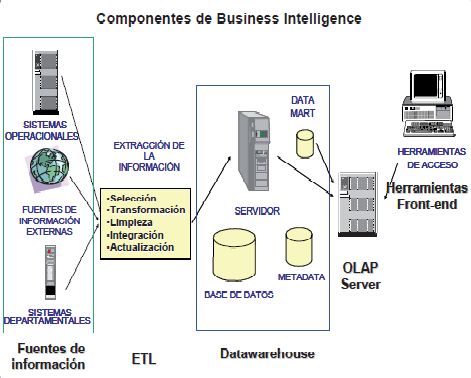
\includegraphics[width=7cm]{imagenes/data.png}

\subsubsection{Principales herramientas de Business Intelligence}
\begin{itemize}
    \item  Generadores de informes: Utilizadas por desarrolladores profesionales para crear informes estándar para grupos, departamentos o la organización. 
    \item   Herramientas de usuario final de consultas e informes: Empleadas por usuarios finales para crear informes para ellos mismos o para otros; no requieren programación. 
    \item   Herramientas OLAP: Permiten a los usuarios finales tratar la información de forma multidimensional para explorarla desde distintas perspectivas y periodos de tiempo. 
    \item   Herramientas de Dashboard y Scorecard: Permiten a los usuarios finales ver información crítica para el rendimiento con un simple vistazo utilizando iconos gráficos y con la posibilidad de ver más detalle para analizar información detallada e informes, si lo desean.
    \item   Herramientas de planificación, modelización y consolidación: Permite a los analistas y a los usuarios finales crear planes de negocio y simulaciones con la información de Business Intelligence. Pueden ser para elaborar la planificación, los presupuestos, las previsiones. Estas herramientas proveen a los dashboards y los scorecards con los objetivos y los umbrales de las métricas.  
    \item   Herramientas datamining: Permiten a estadísticos o analistas de negocio crear modelos estadísticos de las actividades de los negocios. Datamining es el proceso para descubrir e interpretar patrones desconocidos en la información mediante los cuales resolver problemas de negocio. Los usos más habituales del datamining son: segmentación, venta cruzada, sendas de consumo, clasificación, previsiones, optimizaciones, etc.
\end{itemize}

\subsubsection{Plataformas de business intelligence}
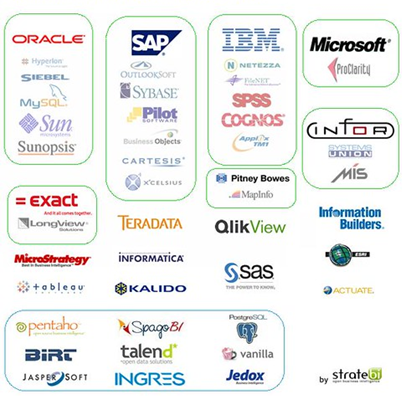
\includegraphics[width=7cm]{imagenes/plataformas.png}
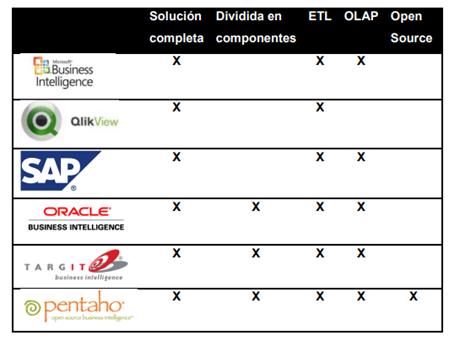
\includegraphics[width=7cm]{imagenes/comparativa.png}

\subsection{Business Analytics}
\subsubsection{Concepto}
Se entiende por business analytics el conjunto de estrategias, tecnologías y sistemas que permiten analizar el rendimiento pasado de una organización para poder predecir comportamientos futuros, así como para detectar patrones ocultos en la información, basadas en datos para extraer inferencias y tomar decisiones calculadas con mayor precisión. certeza. Business Analytics se define como la proceso de explorar, experimentar, simular y resumir datos para extraer información.
\subsubsection{Tipos de analítica}

\begin{itemize}
    \item   Descriptiva: La aplicación de técnicas estadísticas simples que describen lo que es contenidos en un conjunto de datos o base de datos. Ejemplo: Se utiliza un gráfico de barras de edad para representar a los compradores minoristas de una tienda por departamentos que quiere orientar la publicidad a los clientes por edad
    \item   Predictiva: Una aplicación de software estadístico, de información u operaciones avanzadas. métodos de investigación para identificar variables predictivas y construir modelos para identificar tendencias y relaciones que no se observan fácilmente en un análisis descriptivo. Ejemplo: La regresión múltiple se usa para mostrar la relación (o falta de relación) entre la edad, el peso y el ejercicio en venta de alimentos dietéticos. Saber que existen relaciones ayuda a explicar por qué un conjunto de variables independientes influye en las variables dependientes como el negocio rendimiento.
    \item   Prescriptiva: Una aplicación de la ciencia de la decisión, la ciencia de la gestión y las operaciones. metodologías de investigación (técnicas matemáticas aplicadas) para hacer mejor uso de los recursos asignables. Ejemplo: Una tienda departamental tiene un número limitado presupuesto de publicidad para los clientes objetivo. Los modelos de programación lineal pueden ser usados para asignar de manera óptima el presupuesto a varios medios publicitarios.
\end{itemize}

\subsubsection{Dominios de Business Analytics}
Los dominios se refieren a la variedad de actividades dentro de un negocio. El análisis de negocios es construido alrededor (pero no limitado a) los siguientes dominios analíticos:
\begin{itemize}
    \item   Análisis de recursos humanos.
    \item   Análisis de la cadena de suministro.
    \item   Análisis de clientes.
    \item   Análisis de procesos de negocio.
    \item   Análisis financiero.
\end{itemize}

\subsubsection{Tipos de organización BA}

Thomas H. Davenport clasifica las organizaciones en función de su grado de orientación estratégica al business analytics, asimismo, identifica cinco factores críticos a la hora de llevar a la práctica las actividades analíticas en nuestras organizaciones y serán precisamente estos factores críticos los que nos permitirán transitar de un nivel de la pirámide analítica al siguiente.
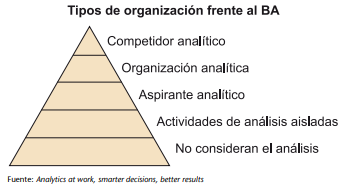
\includegraphics[width=7cm]{imagenes/tipos.png}

\subsubsection{Actividades propias del BA}
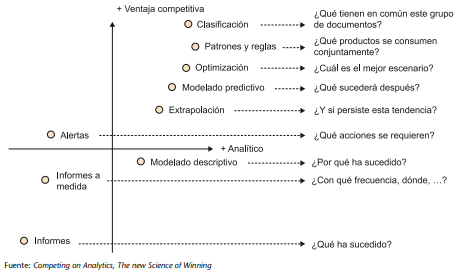
\includegraphics[width=7cm]{imagenes/actividades.png}

\begin{itemize}
    \item   Informes. Se trata de aquellas actividades de exploración de datos que nos permiten interactuar con estos mediante gráficos, estadísticas básicas y vistas.
    \item   Modelado descriptivo. 
    \item   Modelado predictivo. 
    \item   Descubrimiento de patrones y reglas. 
    \item   Clasificación y recuperación de contenidos. 
\end{itemize}

\subsubsection{Relación del Proceso BA y el proceso de toma de decisiones de la organización} 
El proceso BA puede resolver problemas e identificar oportunidades para mejorar el rendimiento empresarial. En el proceso, las organizaciones también pueden determinar estrategias para guiar operaciones y ayudar a lograr ventajas competitivas. Por lo general, la resolución de problemas e identificar oportunidades estratégicas a seguir son tareas de toma de decisiones de la organización.
Este último, la identificación de oportunidades puede verse como un problema de elección de estrategia. requiriendo una solución.  el proceso analítico de negocios tiene una relación inherente con los pasos en los procesos típicos de toma de decisiones de una organización.
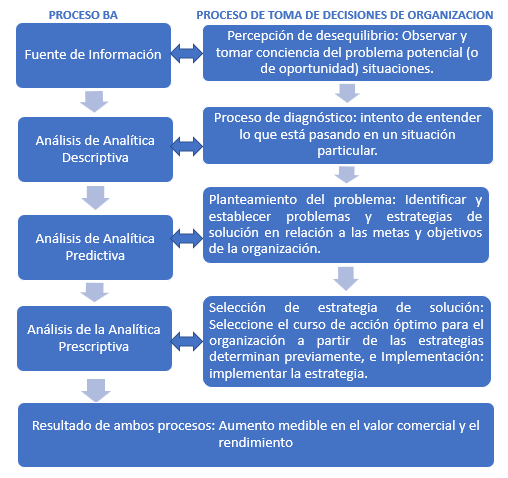
\includegraphics[width=7cm]{imagenes/tomadecisiones.png}
\subsection{Comparativa entre Business Analytics y Business Intelligence}
La principal distinción entre inteligencia de negocio y analitica de negocio es el enfoque en el momento en que ocurren los eventos. BI se centra en eventos actuales y pasados que se capturan en los datos. BA se centra en lo que es más probable que suceda en el futuro.  Esta diferencia se puede resumir en dos preguntas sencillas:
¿Qué está pasando ahora y por qué? (Business Intelligence)
¿Qué pasará después? (Business Analytics) 
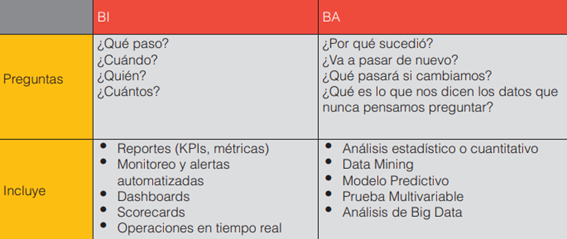
\includegraphics[width=7cm]{imagenes/comparativa1.png}
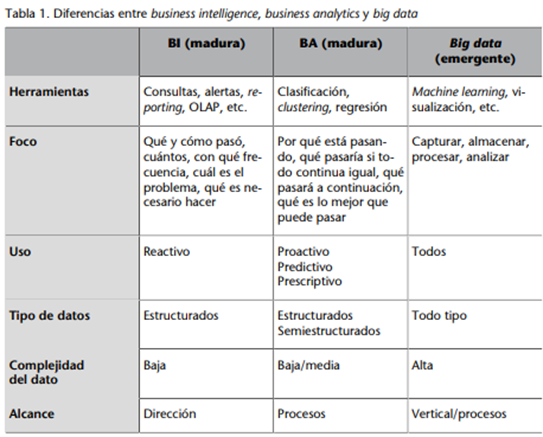
\includegraphics[width=7cm]{imagenes/comparativa2.png}

\section{Conclusiones}
En forma exclusiva, la inteligencia empresarial y el análisis de negocios forman los componentes esenciales requeridos por una empresa para administrar su información de manera efectiva. Las dos terminologías parecen tener similitudes de una manera que hace que los estudiantes deduzcan que están conectados. De hecho, vale la pena reconocer que la analítica es una función de la inteligencia empresarial. La información analizada mediante análisis para predecir el futuro es la misma información obtenida del componente de inteligencia de la empresa. Tanto BI como BA se enfocan en impulsar a la compañía a avanzar enérgicamente En un medio globalizado y audaz como el del mundo empresarial, podemos ver que el entorno en el que la inmensa mayoría de las empresas tiene soportados los procesos de negocio con diferentes sistemas de información y estrategias, los ubica en un mercado tan competitivo como el actual, Hoy se ha convertido en un problema, por lo que la Inteligencia de Negocios se rige como una pieza clave para ser proactivo a la hora de tomar mejores decisiones y de conseguir mejor control de negocio y ventajas que nos diferencien de la competencia



\section{Recomendaciones}
El análisis de datos en un tema obligatorio para el sector financiero. La velocidad a la que cambian y avanzan los sistemas de información obligan a las compañías a adaptarse al cambio, pues no hacerlo puede significar el fracaso. 
Nadeem (Nadeem y Jaffri, 2007) explica que en casos particulares como el sector financiero, fenómenos como la globalización, regulación, fusiones y logros, la competencia desde instituciones no financieras y la innovación tecnológica, influencian la industria de los servicios financieros y obligan a las compañías pertenecientes al sector a repensar sus empresas. Esta es la razón por la que grandes compañías han venido usando software de Inteligencia de Negocios por algunos años, pues les ha ayudado a forjar ventajas competitivas claves a la hora de enfrentarse unas con otras en la rivalidad del mercado.
Con el nuevo escenario, todos los procesos de planeación avanzada de una empresa se integran amparados por una misma práctica, asegurando la participación y colaboración de todas las áreas estratégicas del grupo, como ventas, mercadeo, logística y producción.
 

%----------------------------------------------------------------------------------------
%	REFERENCE LIST
%----------------------------------------------------------------------------------------

\begin{thebibliography}{XXX0000}
	\bibitem  - Business Intelligence: Transformando la forma de hacer negocio a través de los datos. (n.d.). Retrieved from https://www.pwc.com/ve/es/publicaciones/assets/PublicacionesNew/Boletines/Business
	
  \bibitem  - Roig, J. (n.d.). Analítica de negocio. Retrieved from\ http://openaccess.uoc.edu/webapps/o2/bitstream/10609/71345/2/Business
	
  \bibitem  - Business Analytics Principles, Concepts, 
  and Applications. (n.d.). Retrieved from 
  https://ptgmedia.pearsoncmg.com/images/9780133552188/samplepages/0133552187.pdf
	
  \bibitem  - Bag, D. (2016, November 10). Business Analytics. 
  Retrieved March 22, 2022, from ResearchGate website: 
  https://www.researchgate.net/publication/318966560BusinessAnalytics/link/6226d5b184ce8e5b4d0f6f18/download
	
  \bibitem  - En, M., Estratégica, P., Dirección, Y., 
  Tecnología, D., Noemi, G.,  Ventura, V. (n.d.). 
  INTELIGENCIA DE NEGOCIOS BUSINESS INTELLIGENCE (BI) BASE DE 
  DATOS ITI-552 M.C. LEOPOLDO GONZÁLEZ ROSAS. Retrieved from 
  https://basesdatoscms.files.wordpress.com/2012/10/resumen-businessintelligence.pdf
	
  \bibitem  - Cano, J. (n.d.). BUSINESS INTELLIGENCE:
   COMPETIR CON INFORMACIÓN BUSINESS INTELLIGENCE: 
   COMPETIR CON INFORMACIÓN. Retrieved from https://itemsweb.esade.edu/biblioteca/archivo/Business Intelligence competir con informacion.pdf
	
  \bibitem  - Curto, J.,  Pid00238512, D. (n.d.). 
  Introducción a la business intelligence. Retrieved from 
  http://openaccess.uoc.edu/webapps/o2/bitstream/10609/136207/2/Fundamentos
	
  \bibitem  - Carlos, U., De Madrid, I., Autor, C., 
  Cámara, N.,  Director. (2010). ANÁLISIS DE LOS SISTEMAS 
  BUSINESS INTELLIGENCE Y SU APLICACIÓN PRÁCTICA EN LOS PROYECTOS SOFTWARE PROYECTO FIN DE CARRERA. Retrieved from https://core.ac.uk/download/pdf/30043605.pdf
	
  \bibitem  - SINNEXUS (s.f.) Que es Business 
  Intelligence 
  http://sgpwe.izt.uam.mx/files/users/uami/sppc/Business Intelligence/Sinnexus Que es Business Intelligence.pdf
	
  \bibitem  - Medina, L., Plata, E.,  Humberto. (n.d.). 
  Business Intelligence: la información como arma competitiva. 
  Retrieved from https://repositorioacademico.upc.edu.pe/bitstream/handle/10757/333779/112-376-1-PB.pdf?sequence=1isAllowed=y

\end{thebibliography}

%----------------------------------------------------------------------------------------

\end{document}